\documentclass[review]{elsarticle}

\usepackage{amsmath}
\usepackage{amssymb}

\usepackage{soul,color}
\usepackage{textcomp}

\usepackage{lineno,hyperref}
\modulolinenumbers[1]

\newcommand{\tr}[1]{\mathrm{Tr} \left\{ #1 \right\}}
\newcommand{\sx}{I_\mathrm{x}}
\newcommand{\sy}{I_\mathrm{y}}
\newcommand{\sz}{I_\mathrm{z}}
\newcommand{\hdz}{H_\mathrm{dz}}

\journal{Journal of Magnetic Resonance}

%% `Elsevier LaTeX' style
%\bibliographystyle{elsarticle-num}
\bibliographystyle{naturemag}

%%%%%%%%%%%%%%%%%%%%%%%

\begin{document}

\begin{frontmatter}

\title{Many-spin entanglement in multiple quantum NMR with a dipolar ordered initial state}

\author[icp]{E.~B.~Feldman}
\author[icp,msu]{I.~D.~Lazarev} %

\address[icp]{Institute of Problems of Chemical Physics of Russian Academy of Sciences, \\ Chernogolovka, Moscow Region, Russia 142432}
\address[msu]{Faculty of Fundamental Physical-Chemical Engineering, Lomonosov Moscow State University, GSP-1, Moscow, Russia 119991}



\begin{abstract}
Many-spin entanglement is investigated for a gas spin-carrying molecules (atoms) in nanocavities 
in conditions of the multiple quantum (MQ) NMR with a dipolar ordered initial state.
MQ NMR with the dipolar ordered state opens new possibilities for an exploration of many-spin entanglement. 
The second moment of a distribution of intensities of MQ NMR coherences,
which provides a lower bound of the quantum Fisher information, 
was used for an estimation of the number of entangled spins. 
Many-spin entanglement is investigated at different temperatures and different numbers of spins in the system under consideration.
\end{abstract}

\begin{keyword}
multiple quantum (MQ) NMR \sep  
quantum correlations \sep 
quantum Fisher information \sep 
entanglement, nano-pore \sep 
MQ NMR coherence \sep 
second moment, temperature \sep 
dipolar ordered state \sep 
two-pulse Broekaert-Jeener sequence
\end{keyword}

\end{frontmatter}

\linenumbers

\section{Introduction}
\label{sec:1}

Entanglement~\cite{Nielsen_2009} is a very important quantum conception, which is responsible in particular, for advantages of quantum computers over their classical counterparts.
Recently demonstrated quantum supremacy using a programmable superconducting processor~\cite{Arute2019} is also connected with entanglement which is absent in classical physics.
Among numerous methods of an investigation of entanglement we concentrate on multiple quantum (MQ) NMR in solids~\cite{Baum_1985}, which was widely used to characterize entanglement in binary systems~\cite{Furman_2008,Furman_2009,Fel_dman_2008,Fel_dman_2012}. 
It turned out that the MQ NMR spectroscopy~\cite{Baum_1985} allows us to extract also information about many-spin entanglement~\cite{G_rttner_2018}, 
if one attracts for the analysis the quantum Fisher information~\cite{T_th_2014,Pezz__2018}.

The quantum Fisher information describes quickness of changing quantum states determined by the density matrix at changing some parameter. 
In MQ NMR spectroscopy that parameter is the phase increment between the radio-frequency (rf) pulses irradiating the system on preparation and mixing periods of the MQ NMR experiment~\cite{Baum_1985} in proportional to the evolution time.
That procedure leads to a separation of the signals,
corresponding to the MQ NMR coherences of different orders, and obtaining the total MQ NMR spectrum.
Using the quantum Fisher information (QFI)~\cite{Liu_2014} for an analysis of the MQ NMR spectra one can extract very important information about many-spin entanglement.
The point is that there is a relation between the second moment of the MQ NMR spectrum~\cite{Khitrin_1997} and the quantum Fisher information~\cite{G_rttner_2018,Doronin_2019}.
Moreover the second moment of the MQ NMR spectrum provides a lower bound on the quantum Fisher information~\cite{G_rttner_2018}.
It means that the MQ NMR spectroscopy is a valuable method for solving quantum information problems.

Many-spin entanglement was investigated~\cite{Doronin_2019} on a nonspherical nanopore filled with a gas of spin-carrying molecules in a strong external magnetic field~\cite{Baugh_2001,Doronin_2009}.
The thermal equilibrium initial state of the system was determined by the one-spin Zeemann interaction with the external magnetic field~\cite{Doronin_2007a}.
It is also possible to investigate many-spin entanglement when the same system is initially prepared in the dipolar ordered state~\cite{Goldman_1970} using either the adiabatic demagnetization method in a rotating reference frame (RRF)~\cite{Goldman_1970,Slichter_1961} or the two-pulse Broekaert-Jeener sequence~\cite{Goldman_1970,Jeener_1967}.
The MQ NMR dynamics with this initial state have been simulated both in small spin-systems~\cite{Doronin_2007a,Doronin_2007b} and in the system consisting of 200-600 spin-carrying molecules (atoms) filled in a nanopore~\cite{Doronin_2011}.
The approaches developed for those investigations are restricted by high temperatures and cannot be applied in order to study many-spin entanglement.

In the present article we consider an intermediate temperature case with low Zeemann temperatures and high dipolar ones. 
Nuclear magnetic ordering~\cite{Abragam_1982} is outside our consideration.
Notice also that the two-pulse Broekaert-Jeneer experiment~\cite{Jeener_1967} was performed in the high temperature case.
We prove theoretically that the experiment~\cite{Jeener_1967} can be realized also for the intermediate temperature case of the article. 
It was shown~\cite{Doronin_2011} that in the MQ NMR experiment with the dipolar ordered initial state MQ NMR coherences emerge faster 
than in the MQ NMR experiment with the thermal equilibrium initial state in a strong external magnetic field.
It is important for many-spin entanglement investigations, because they are connected with calculations of the second moment of the distribution of MQ NMR coherences. 
It is also very important for an investigation of the spreading correlation~\cite{Baugh_2001,Baum_1986,S_nchez_2014,Munowitz_1987} and localization effects~\cite{Alvarez_2015,Wei_2018}.
At that the spreading rate can be described through out-of-time ordered correlations which are connected with the distribution of MQ NMR coherences. 

The present paper investigates many-spin entanglement using the MQ NMR spectrum of spin-carrying atoms (molecules) in a nanopore when the system is prepared in the dipolar ordered state.
In Sec.~\ref{sec:2} the theory of MQ NMR dynamics at low Zeemann and high dipolar temperatures is developed.
An analytical solution for the MQ NMR dynamics of a three-spin system is obtained at such temperatures in Sec.~\ref{sec:3}.
The second moment of the MQ NMR spectrum as a measure of many-spin entanglement is considered in Sec.~\ref{sec:4}.
The dependence of many-spin entanglement on the dipolar temperature and the number of spins in the system is investigated in Sec.~\ref{sec:5}.
We briefly summarize our results in the concluding Sec.~\ref{sec:6}.
In Appendix we show that the two-pulse Broekaert-Jeener sequence can be used in the case when the Zeemann temperature is low and the dipole one is high.



\section{Theory of MQ NMR dynamics in a nanopore at low Zeemann and high dipolar temperatures}
\label{sec:2}

MQ NMR dynamics in a nanopore governs the Hamiltonian~\cite{Doronin_2019,Doronin_2009} 
%
\begin{equation}
    \label{eq:1}
    H_{\mathrm{MQ}} = - \dfrac{D}{4} \left[
        \left(I^{+}\right)^{2} 
        + \left(I^{-}\right)^{2} 
    \right] ,
\end{equation}
%
where 
%
\begin{equation}
    \label{eq:2}
    I^{\pm} = \sum\limits_{j=1}^{N} I_{j}^{\pm},
\end{equation}
%
$N$ is the number of the spins in the nanopore, $I^{\pm}_{j}$ are the raising or lowering operators of spin $j$, and $D$ is the dipolar coupling constant averaged by the fast molecular diffusion of spin-carrying atoms (molecules) in nanopores.
We underline that the dipolar coupling constant $D$ is the same for all pairs of interacting spins in the nanopore~\cite{Doronin_2019,Doronin_2009}.
The density matrix $\rho(\tau)$ on the preparation period of the MQ NMR experiment~\cite{Baum_1985} can be obtained from the Liouville evolution equation~\cite{Goldman_1970,Abragam_1982} 
%
\begin{equation}
    \label{eq:3}
    i\dfrac{\mathrm{d}\rho(\tau)}{\mathrm{d}\tau} = \left[
    H_\mathrm{MQ},\rho(\tau)
    \right]
\end{equation}
%
with the initial thermodynamic equilibrium density matrix 
%
\begin{equation}
    \label{eq:4}
       \rho(0) = \rho_\mathrm{eq} = \dfrac{1}{Z}
       e^{
            \frac{\hslash \omega}{k} \alpha_\mathrm{z} I_\mathrm{z} 
            + \frac{\hslash }{k} \beta_\mathrm{d} H_\mathrm{dz}
        },
\end{equation}
%
where 
$Z = \mathrm{Tr} \left\{ e^{\frac{\hslash \omega}{k} \alpha_\mathrm{z} I_\mathrm{z} + \frac{\hslash  }{k} \beta_\mathrm{d} H_\mathrm{dz}} \right\}$ is the partition function, 
$\hslash$ and $k$ are the Plank and Boltzmann constants, 
$\omega_{0}$  is the Larmor frequency , $I_\mathrm{z}$ is the operator of the projection of the total spin angular momentum on the z-axis, 
which is directed along the strong external magnetic field,  
$H_\mathrm{dz}$ is the secular part of the dipole-dipole interaction~(DDI) Hamiltonian in a strong external magnetic field, and $\alpha_\mathrm{z}$, $\beta_\mathrm{d}$ are the inverse Zeemann and dipolar temperatures. 
We will consider the case when the Zeemann temperature is low $({\frac{\hslash \omega}{k} \alpha_\mathrm{z}}\gg 1)$ 
and the dipolar temperature is high $\left( \frac{\hslash{D}}{k}\beta_\mathrm{d} \ll 1\right)$.
For concreteness we suppose that $\omega_{0} = 2\pi \cdot 500 \cdot 10^{6}$~s$^{-1}$ and $D = 2\pi \cdot 10^{4}$~s$^{-1}$.
In Appendix we proved that the two-pulse Broekaert-Jeener sequence~\cite{Goldman_1970,Jeener_1967} results in the dipolar ordered state even at the low Zeemann temperature.
The adiabatic demagnetization~\cite{Goldman_1970,Slichter_1961} is the second method of preparing the system in the dipolar ordered state.
Using those methods we can obtain the system in the thermodynamic equilibrium state with the density matrix
%
\begin{equation}
    \label{eq:5}
    \rho_i = \frac{1}{Z_i} e^\frac{\hslash\beta_\mathrm{d} \hdz}{k}
    \approx \frac{1}{Z_i}(1 + \frac{\hslash\beta_\mathrm{d}}{k} H_\mathrm{dz}),
\end{equation}
%
where the partition function
%
\begin{equation}
    \label{eq:6}
	Z_i = \mathrm{Tr} \left\{ e^\frac{\hslash\beta_\mathrm{d} \hdz}{k} \right\} \approx 2^{N}.
\end{equation}
%
MQ NMR dynamics in the nanopore will be investigated on the basis of Eq.~(\ref{eq:3}) with the initial state of Eq.~(\ref{eq:5}).
It is also significant that the Hamiltonian $H_{dz}$ is partially averaged by the fast molecular diffusion in the nanopore and the averaged Hamiltonian can be written as \cite{Fel_dman_2004,Doronin_2011}
%
\begin{equation}
    \label{eq:7}
    H_\mathrm{dz} = \dfrac{D}{2} (3 I^{2}_{z} - I^{2}) , % ?
\end{equation}
%
where $I^{2}$ is the square of the spin angular momentum.

The averaged over the equilibrium density matrix of Eq.~(\ref{eq:5})the resulting signal $G(\tau,\phi)$ after the preparation, evolution and mixing periods of the MQ NMR experiment~\cite{Baum_1985} can be written as~\cite{Doronin_2019} 
%
\begin{equation}
    \begin{split}
        \label{eq:8}
        G(\tau,\phi) 
        & = \mathrm{Tr}\left\{
            e^{i H_\mathrm{MQ} \tau} e^{i\phi I_\mathrm{z}} e^{-i H_\mathrm{MQ}\tau} 
            \rho_i 
            e^{i H_\mathrm{MQ} \tau} e^{-i \phi I_\mathrm{z}} e^{-i \phi H_\mathrm{MQ} \tau} 
            \rho_i 
        \right\} \\
        & = \mathrm{Tr} \left\{
        e^{i \phi I_\mathrm{z}}
        \rho(\tau) 
        e^{-i \phi I_\mathrm{z}} 
        \rho(\tau) 
        \right\},
    \end{split}
\end{equation}
%
where
%
\begin{equation}
    \label{eq:9}
    \rho(\tau) 
    = e^{-i H_\mathrm{MQ} \tau } 
    \rho_i 
    e^{i H_\mathrm{MQ} \tau}
\end{equation}
%
is the solution of Eq.~(\ref{eq:3}) at the initial condition of Eq.~(\ref{eq:5}).
It is convenient to expand the spin density matrix, $\rho(\tau)$, in series as
%
\begin{equation}
    \label{eq:10}
    \rho(\tau) = \sum\limits_n \rho_n(\tau),
\end{equation}
%
where $\rho_{n}(\tau)$ is the contribution to $\rho(\tau)$ from the MQ coherence of the $n$-th order~\cite{Fel_dman_1996}.
Then the function $G(\tau,\phi)$ of Eq.~(\ref{eq:8}) can be rewritten as 
%
\begin{equation}
    \label{eq:11}
    G(\tau,\phi) 
    = \sum\limits_n e^{i n \phi} \mathrm{Tr} \left\{ 
        \rho_{n}(\tau) \rho_{-n}(\tau) 
    \right\},
\end{equation}
%
where we took into account that
%
\begin{equation}
    \label{eq:12}
    \left[ I_{\mathrm{z}},\rho_n(\tau) \right] = n \rho_n(\tau)
\end{equation}
%
It is necessary for further calculations to introduce the normalized intensities $J_{n}(\tau)$ $(n=0, \pm 2, \pm 4, \cdots)$ of the MQ NMR coherences
%
\begin{equation}
    \label{eq:13}
    J_{n}(\tau) = \dfrac{\mathrm{Tr} \left\{
    \rho_{n}(\tau) \rho_{-n}(\tau) 
    \right\}} 
    {\mathrm{Tr} \left\{\rho^2_{i} \right\}}
\end{equation}
%
Using Eqs.~(\ref{eq:9})~(\ref{eq:10}) one can verity that 
%
\begin{multline}
    \label{eq:14}
    \sum\limits_{n} J_{n}(\tau)
    = \dfrac{
        \mathrm{Tr} \left\{
            \sum_{n} \rho_{n}(\tau) \rho_{-n}(\tau)
        \right\}}
    {\mathrm{Tr} \left\{ \rho^2_{i} \right\}} 
    = \dfrac{
        \mathrm{Tr} \left\{
            \sum_{\mathrm{m,n}} \rho_n(\tau)\rho_m(\tau)
    \right\}}
    {\mathrm{Tr} \left\{\rho^2_{i}\right\}}
    \\
    = \dfrac{
        \mathrm{Tr}\left\{\rho^2(\tau)\right\}
    }
    {
        \mathrm{Tr}\left\{\rho^2_{i}(\tau)\right\}
    }
    = \dfrac{
        \mathrm{Tr} \left\{ 
            e^{-i H_\mathrm{MQ} \tau} 
            \rho^{2}_{i}
            e^{i H_\mathrm{MQ} \tau} 
        \right\}
    }
    {
        \mathrm{Tr} \left\{ \rho_{i}^{2} \right\}
    } 
    = 1
\end{multline}
%
One can conclude from Eq.~(\ref{eq:14}) that the sum of the MQ NMR coherences is conserved on the preparation period of the MQ NMR experiment~\cite{Baum_1985}.

The basis consisting of eigenstates of the operator $I_\mathrm{z}$ (so called the multiplicative basis) is widely used for numerical calculations of MQ NMR dynamics~\cite{Zhang_2009}.
Due to the fast expansion of the Hilbert space with the growth of the number of spins such calculations are possible only for systems with a small number of spins.
That approach is not suitable for investigations of many-spin entanglement.
Since the Hamiltonian $H_{MQ}$ of Eq.~(\ref{eq:1}) commutes with the square of the total spin angular momentum $\hat I^2$ 
it is possible to use the basis consisting of the common eigenstates of $\hat I^2$ and $I_\mathrm{z}$ in order to study MQ NMR dynamics as was done in Ref.~\cite{Doronin_2009,Doronin_2011,Doronin_2019}.
In this basis the Hamiltonian $H_{MQ}$ and the initial density matrix of Eq.~(\ref{eq:5}) (see also Eq.~(\ref{eq:7})) consist of blocks corresponding to different values of the spin angular momentum~\cite{Doronin_2009}.
Then the investigation of MQ NMR dynamics can be reduced to solving a set of problems of less dimensions.

Since the Hamiltonian $H_{MQ}$ of Eq.~(\ref{eq:1}) commutes with the operator $e^{i\pi I_\mathrm{z}}$, $2^N \times 2^N$ Hamiltonian matrix is reduced to two $2^{N-1} \times 2^{N-1}$ submatrices~\cite{Doronin_2009}.
For odd $N$, both submatrices give the same contribution to the MQ NMR coherences, and one should solve the problem using only one $2^{N-1} \times 2^{N-1}$ submatrix and double the obtained intensities. 
In our calculations we take only odd numbers of spin.
Using this method one can investigate MQ NMR dynamics in systems consisting of hundred spins.

\section{Analytical solution for MQ NMR dynamics for a three-spin system in a nanopore in dipolar ordered state}
\label{sec:3}

\begin{figure}
    \centering
  	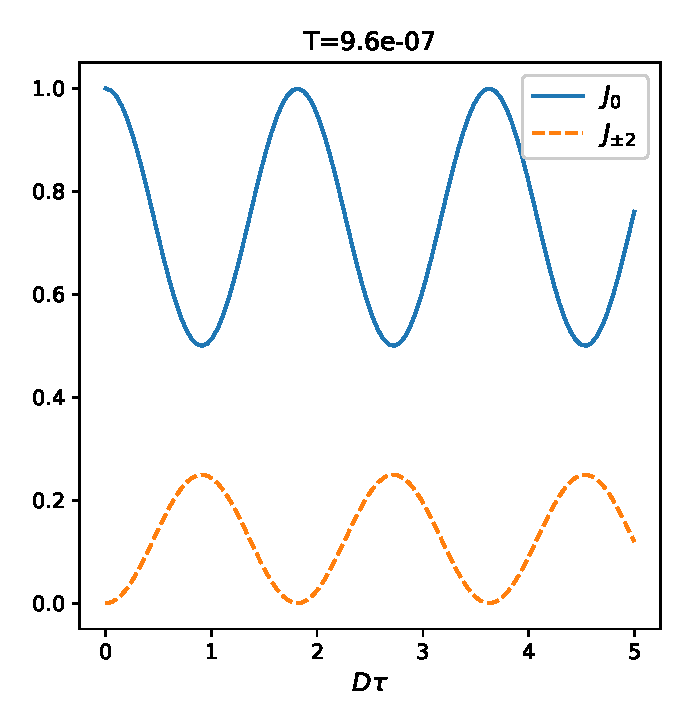
\includegraphics[width=0.5\linewidth]{coherences_n3_beta5.eps}
	\caption{
	    Intensities of MQ NRM coherenes $J_{n}$ ($n=0, 2$) in a nanopore with $N=3$.
	}
	\label{fig:1}
\end{figure}

Obtaining the exact solution for MQ NMR dynamics for a three-spin system in the dipolar ordered state in a nanopore is analogously to the case considered in~\cite{Doronin_2019} for the initial thermodynamic equilibrium in a strong external magnetic field. 
We does not use here the high temperature approximation~\cite{Goldman_1970}.

The Hamiltonian $H_{MQ}$ of Eq.~(\ref{eq:1}) consists here of the two blocks for two possible values of spin angular momentum $(I^2 = S(S+1),  \quad S=3/2,1/2)$.
Those blocks, the corresponding eigenvalues and eigenstates are given in~\cite{Doronin_2019}.
The density matrix of the system consists also of the two blocks $\rho^{3/2}(\tau)$, $\rho^{1/2}(\tau)$, and 
%
\begin{equation}
    \label{eq:15} 
    \rho^{3/2}(0) = \dfrac 1 Z
    \begin{pmatrix}
        e^{\frac{3b}{2}} & 0 & 0 & 0 
        \\
        0 & e^{\frac{-3b}{2}} & 0 & 0 
        \\
        0 & 0 & e^{-\frac{-3b}{2}} & 0 
        \\
        0 & 0 & 0 & e^{\frac{3b}{2}}
    \end{pmatrix}, 
    \quad
    \rho^{1/2}(0) = \dfrac 1 Z
    \begin{pmatrix}
       	1 & 0 
        \\
        0 & 1
    \end{pmatrix}
\end{equation}
%
where $b = \dfrac{\hslash D}{k\mathrm{T}}$and $T$ is the temperature.
After simple calculations one can obtain the density matrices $\rho^{3/2}(\tau)$ and $\rho^{1/2}(\tau)$ 
which allow us to find intensities of the MQ NMR coherences.

Only the MQ NMR coherences of the zeroth and plus/minus second orders appear in the considered systems. 
The intensities of these coherences are
%
\begin{equation}
    \begin{split}
        \label{eq:16}
        J_0(\tau) & = 1 
        - \dfrac 1 2 \tanh^2\left( \dfrac{3b}{2} \right)
            \sin^2 \left( \sqrt{3} Dt \right), 
        \\
        J_{\pm2}(\tau) & = \dfrac{1}{4} 
            \tanh^2 \left( \dfrac{3b}{2} \right)
            \sin^2 \left( \sqrt{3} Dt \right)
    \end{split}
\end{equation}
%
The sum of intensities of Eq.~(\ref{eq:16}) equals one in accordance with Eq.~(\ref{eq:14}).
The dependencies of the calculated intensities $J_{n}(\tau)$ $(n=0,2)$ on the evolution time are shown in Fig.~(\ref{fig:1}).



\section{Second moment of the MQ NMR spectrum as a measure of many-spin entanglement}
\label{sec:4}

The expression~(\ref{eq:8}) for the MQ NMR signal $G(\tau,\phi)$ can be expanded in series over the phase increment $\phi$:
%
\begin{equation}
    \begin{split}
        \label{eq:17}
        G(\tau,\phi)  
        & = \mathrm{Tr} \left\{ 
            \rho(\tau) e^{i \phi I_\mathrm{z} }
            \rho(\tau) e^{-i\phi I_\mathrm{z}}
        \right\}  \\
        & = \mathrm{Tr} \left\{ \rho^2(\tau) \right\} 
        - \phi^2 \mathrm{Tr} \left\{ 
            \rho^2(\tau) I^2_\mathrm{z} 
            - (\rho(\tau) I_\mathrm{z})^2
        \right\} 
        + O(\phi^3)
    \end{split}
\end{equation}
%
It is possible to prove~\cite{Girolami_2017} that the quantum Fisher information $F_\mathrm{Q}(\rho,I_\mathrm{z})$~\cite{Helstrom_1976}
%
\begin{equation}
    \label{eq:18}
    F_\mathrm{Q}(\rho,I_\mathrm{z}) \geq 4 \mathrm{Tr} \left\{ \rho^2 I^2_\mathrm{z} - (\rho I_\mathrm{z})^2 \right\}
\end{equation}
%
At the same time, it is easily to verify that $2 \mathrm{Tr} \left\{ \rho^2(\tau) I_\mathrm{z}^2 - \left( \rho(\tau) I_\mathrm{z} \right)^2 \right\}$ equals to the second moment $M_2$ of the distribution of intensities of the MQ NMR coherences~\cite{Khitrin_1997}
%
\begin{equation}
    \label{eq:19}
    M_2 = \sum_{n} n^2 J_n (\tau) ,
\end{equation}
%
where $J_n(\tau)$ ($n=0,\pm 2, \pm 4, \cdots$) is determined by Eq.~(\ref{eq:13}).
Thus, the second moment of the MQ NMR spectrum provides a low bound on the quantum Fisher information $F_\mathrm{Q}(\rho,I_\mathrm{z})$
It was also shown~\cite{T_th_2014,Pezz__2018} that if
%
\begin{equation}
    \label{eq:20}
    F_\mathrm{Q} (\rho,I_\mathrm{z}) > n k^2 + (N - n k)^2,
\end{equation}
%
where $n$ is the integer part of {N/k}, then the system with the density matrix $\rho(\tau)$ is $k+1$-spin entangled~\cite{Pezz__2009,Hyllus_2012,T_th_2012}.
The results of the numerical analysis of many-spin entanglement in the system of spin-carrying molecules (atoms) initially prepared in the dipolar ordered state are presented in the following section.



\section{Numerical analysis of many-spin entanglement at different temperatures and the numbers of spins in the system}
\label{sec:5}

\begin{figure}
  	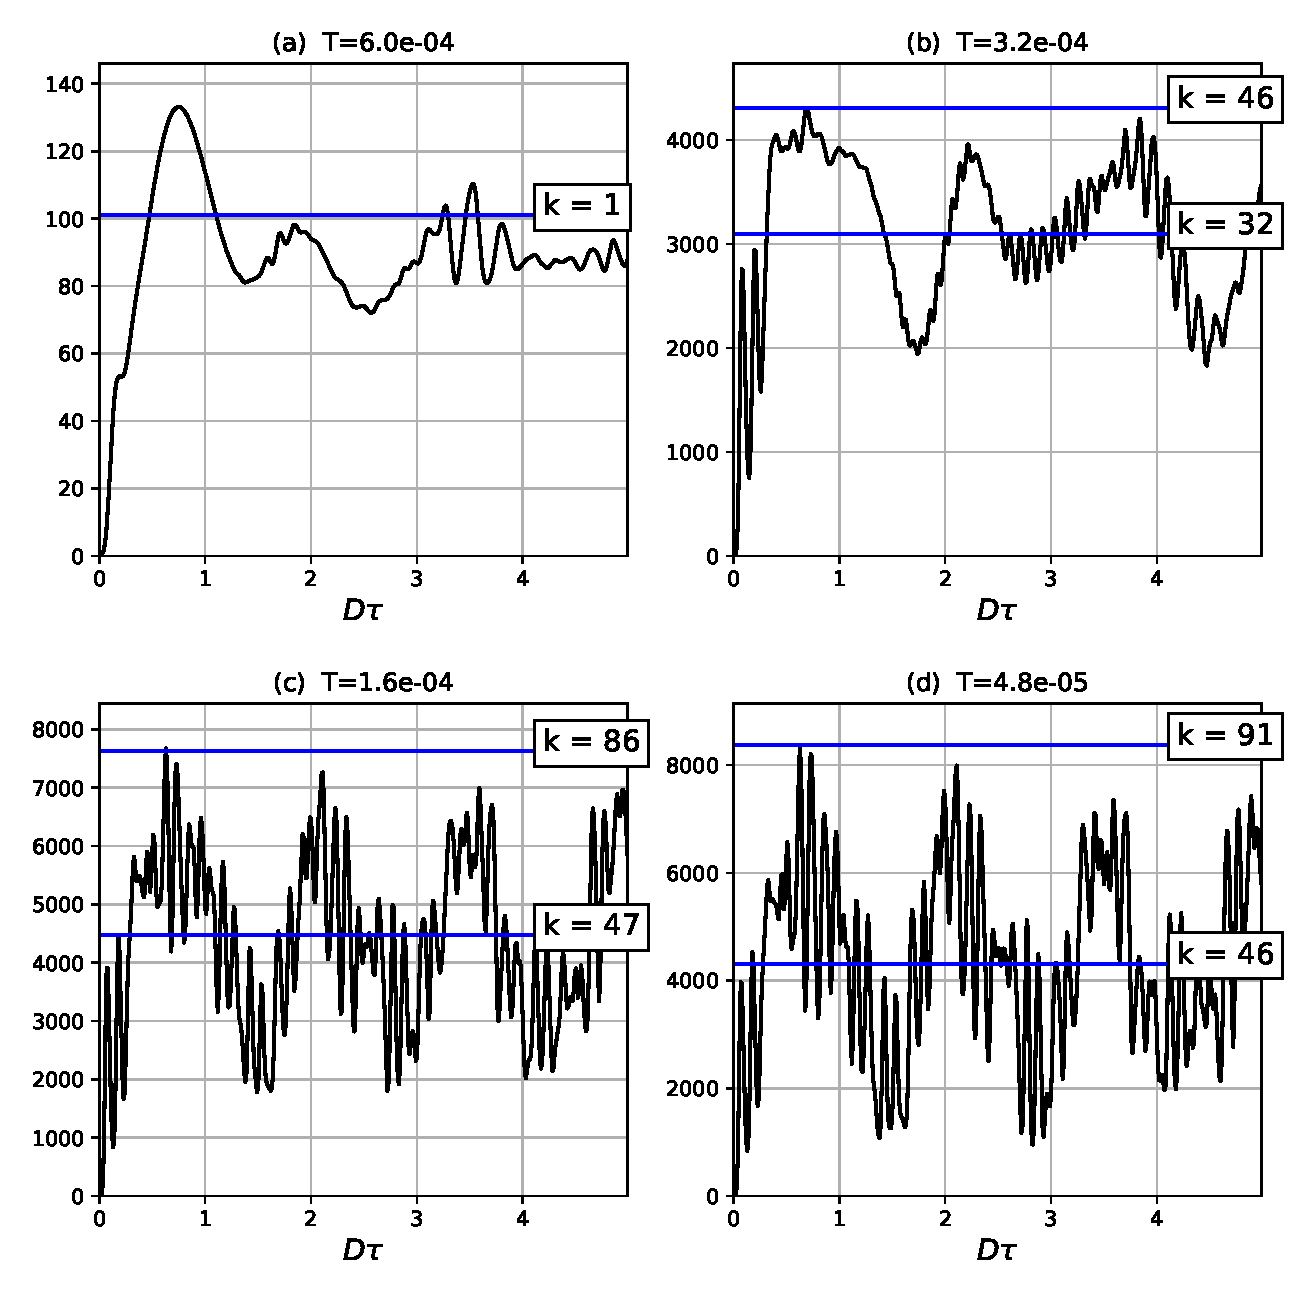
\includegraphics[width=0.95\linewidth]{fisher_low_bound_n101.eps}
	\caption{
	    The dependence of the low bound of the quantum Fisher Information $F_\mathrm{Q} = 2 M_{2}$ 
	    on the dimensionless time $D\tau$ at $N=101$, 
	    a) $T=6\cdot10^{-4}$~K, the inequality~(\ref{eq:20}) yields the region of pair entanglement (k+1=2), the region is above the horizontal line; 
	    b) $T=3.2\cdot10^{-4}$~K, the region of the many-spin entanglement is a strip bounded by the horizontal lines with~$k=32$~and~$k=46$; 
	    c) $T = 1.6\cdot10^{_4}$~K, the horizontal lines ($k=47$ and k=$86$) bound the strip with many spin enatnglement;
	    d) $T=4.8\cdot10^{-5}$~K, entangled clusters with $47-92$ spins emerge.
	}
	\label{fig:2}
\end{figure}

The considered model of the spin-carrying molecules (atoms) in a nanopore in the dipolar ordered states expands possibilities of an investigation of many-spin entanglement in comparison to the analogous model~\cite{Doronin_2019}
when the system was initially in the thermodynamic equilibrium in a strong external magnetic field.
The model~\cite{Doronin_2019}  is restricted for investigation of the time evolution of the system
because the stationary distribution of MQ NMR coherences establishes very quickly~\cite{Doronin_2009}.
The temperature dependence of many-spin entanglement occurs in the model~\cite{Doronin_2019} in a very narrow temperature interval.
For example, all spins are entangled in the system consisting of 201 spins at temperature $T=6.856\cdot10^{-3}$~K~\cite{Doronin_2019}.

The time dependence of the quantum Fisher information in the system consisting of 101 spins is presented in Fig.~(\ref{fig:2}) at different temperatures. 
One can see from Fig.~(\ref{fig:2}a) that only the pair entanglement exists at temperature $T=6\cdot10^{-4}$~K.
At the temperature $T=3.2\cdot10^{-4}$ one can see a strip Fig.~(\ref{fig:2}b), in which the inequality~(\ref{eq:20}) can be satisfied when ${32}\leq {k}\leq{46}$.
Thus, there is many-spin entanglement in spin clusters consisting of 33-47 spins at temperature $3.2\cdot10^{-4}$~K.
When the temperature decreases, the width of the strip, in which many-spin entanglement exists, increases. 
At temperature $T=1.6\cdot10^{-4}$~K (Fig.~(\ref{fig:2}c)) clusters of 48-87 entangled spins emerge, and at temperature $T=4.8\cdot10^{-5}$~K (Fig.~(\ref{fig:2}d)) we have 47-92 entangled spins.

\begin{figure}
  	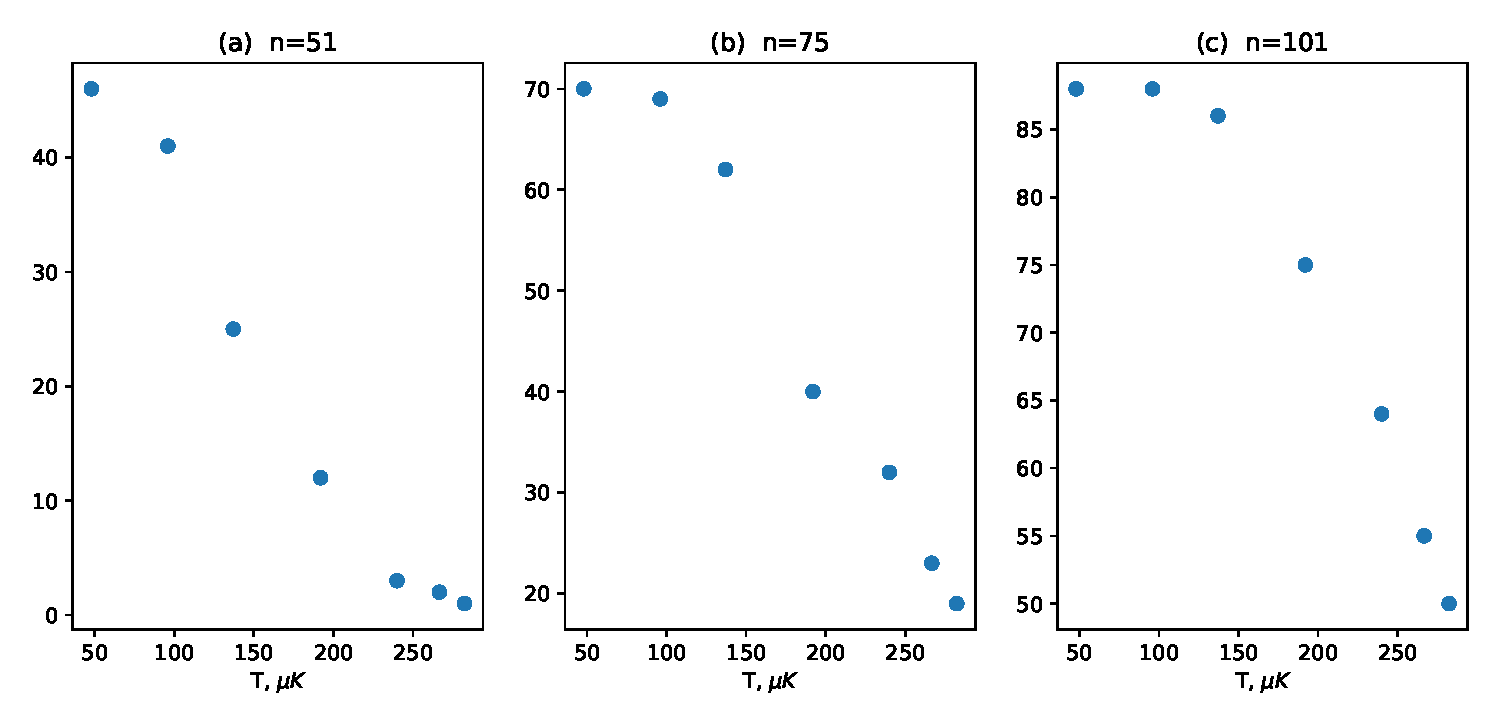
\includegraphics[width=0.95\linewidth]{entangled_spins_by_n.eps}
	\caption{
	    The dependence of the maximal number of the entangled spins,
	    averaged over the evolution time $(0 \leq D\tau \leq 3)$, 
	    on the temperature at a) $N=51$; b) $N=75$; c) $N=101$.
	}
	\label{fig:3}
\end{figure}

The dependence of the maximal number of the entangled spins averaged over the evolution time $({0}\leq \mathrm{D}\tau\leq{3})$, on the temperature at different numbers of spins in a nanopore is presented in Fig.~(\ref{fig:3}).
The maximal number of entangled spins decreases when the temperature increases. 
The maximal number of entangled spins increases when the number of spins in the nanopore increases also, because the system in the nanopore gets more dense. 



\section{Conclusion}
\label{sec:6}

We investigated many-spin entanglement in the system of spin-carrying molecules (atoms) filled in the non-spherical nanopore, initially prepared in the dipolar ordered state, in the conditions of the MQ NMR spectroscopy .
The dependence of many-spin entanglement on the temperature and the number of spins in the nanopore were investigated.

We believe that the MQ NMR spectroscopy is a subtle and useful method for investigations of different quantum information problems.
In particularly, it is a very effective method for exploration of quantum entanglement.



\section{Acknowledgements}
This work was performed as a part of a state task, State Registration No. 0089-2019-0002. 
This work was partially supported by the Russian Foundation for Basic Research (Grants Nos. 20-03-00147, 19-32-80004). 
I.L. acknowledges support from the Advancement of Theoretical Physics and Mathematics BASIS No. 19-1-5-130-1.



\appendix
\section{The two-pulse Broekaert-Jeener experiment at the low Zeemann and high dipolar temperatures.}

Initially the system is in the thermodynamic equilibrium state in the strong external magnetic field with the density matrix
%
\begin{equation}
    \label{eq:a1}
   \sigma_{i} = \dfrac{e^{\beta_\mathrm{L} \omega_{0} I_\mathrm{z}}}{Z_{i}} ,
   \quad
   Z_{i} = \mathrm{Tr}\left\{e^{\beta_\mathrm{L} \omega_{0} I_\mathrm{z}} \right\}
\end{equation}
%
After the first resonance rf x-pulse one has
%
\begin{equation}
    \label{eq:a2}
    \sigma'(0) = e^{ i \frac \pi 2 I_\mathrm{x}}
    \sigma_{i}
    e^{-i \frac \pi 2 I_\mathrm{x}}
    = \dfrac{e^{\beta_\mathrm{L} \omega_{0} I_\mathrm{y}}}{Z_{i}}  .
\end{equation}
%
Then the system evolves freely time $\tau$ 
and one applies the second resonance y-pulse rotating spins by angle $\theta$ around the y-axis of the RRF.
As a result, one obtains that
\begin{equation}
    \label{eq:a3}
    \sigma'(\tau) 
    = \dfrac{
      e^{-i \theta I_\mathrm{y}} e^{-i H_\mathrm{dz} \tau} 
      e^{\beta_\mathrm{L} \omega_{0} I_\mathrm{y}}
      e^{i H_\mathrm{dz} \tau} e^{i \theta I_\mathrm{y}}
    }{Z_{i}}. 
\end{equation}
%
After time $T_2$ ($T_2$ is the spin relaxation time \cite{Goldman_1970}) the system achieves the thermodynamic equilibrium state
\begin{equation}
    \label{eq:a4}
    \sigma_{f} 
    = \dfrac{ e^{\alpha \omega_{0} I_\mathrm{z} + \beta H_\mathrm{dz}} }{Z_f},
\end{equation}
%
where $\alpha$ and $\beta$ are the inverse Zeeman and dipolar temperatures.
It is evident that the system has the single equilibrium state 
and the temperatures $\alpha$ and $\beta$ are also single.
Those temperatures can be obtained from the conservation laws
\begin{align}
    \label{eq:a5}
    \mathrm{Tr} \left\{ I_\mathrm{z} \sigma'(\tau) \right\}
    & = \mathrm{Tr} \left\{ I_\mathrm{z} \sigma_{f}(\tau) \right\}
    \\
    \label{eq:a6}
    \mathrm{Tr} \left\{ H_\mathrm{dz} \sigma'(\tau) \right\}
    & = \mathrm{Tr} \left\{ H_\mathrm{dz} \sigma_{f}(\tau) \right\}
\end{align}
%
One can rewrite $\mathrm{Tr} \left\{ I_\mathrm{z} \sigma'(\tau) \right\}$ as 
%
\begin{multline}
    \label{eq:a7} 
    \tr{I_\mathrm{z} \sigma'(\tau)}
    =  \dfrac{1}{Z_{i}} \tr{
        e^{i \theta \sy} \sz e^{-i \theta \sy}
        e^{-i \hdz \tau} e^{\beta_\mathrm{L} \omega_{0} \sy} e^{i \hdz \tau}
    } 
    \\
    = \dfrac{1}{Z_i} \tr{
        \left( \cos(\theta) \sz - \sin(\theta) \sx \right) 
        e^{-i \hdz \tau} e^{\beta_\mathrm{L} \omega_{0} \sy} e^{i \hdz \tau}
    }
    \\
    = \dfrac{1}{Z_i} \tr{
        e^{-i \pi \sy}  
        \left( \cos(\theta) \sz - \sin(\theta) \sx \right) 
        e^{-i \hdz \tau} e^{\beta_\mathrm{L} \omega_{0} \sy} e^{i \hdz \tau}
        e^{i \pi \sy}  
    }
    \\
    = - \dfrac{1}{Z_i} \tr{
        \left( \cos(\theta) \sz - \sin(\theta) \sx \right) 
        e^{-i \hdz \tau} e^{\beta_\mathrm{L} \omega_{0} \sy} e^{i \hdz \tau} 
    } = 0
\end{multline}
%
In~(\ref{eq:a7} we took into account that $\left[ e^{-i \pi \sy}, \hdz \right] = 0$.
Since we consider the case of a high dipolar temperature it is possible for rewrite~(\ref{eq:a5}) as
\begin{equation}
    \label{eq:a8}
    0 = \dfrac{1}{Z_f} \tr{ \sz e^{\alpha \omega_0 \sz}}
    + \dfrac{\beta}{Z_f} \tr{\sz e^{\alpha \omega_0 \sz} \hdz}.
\end{equation}
%
Notice that $\tr{\sz} = \tr{\sz\hdz} = 0$. It means that $\alpha = 0$ satisfies Eq.~(\ref{eq:5}). 
Thus we obtain the dipolar ordered state in the considered case.

%%%%%%%%%%%%%%%%%%%%%%%%%%%%%
\bibliography{bibliography}
\end{document}
